\documentclass[]{article}
\usepackage{amssymb,amsmath}
\usepackage{ifxetex,ifluatex}
\ifxetex
  \usepackage{fontspec,xltxtra,xunicode}
  \defaultfontfeatures{Mapping=tex-text,Scale=MatchLowercase}
  \newcommand{\euro}{€}
\else
  \ifluatex
    \usepackage{fontspec}
    \defaultfontfeatures{Mapping=tex-text,Scale=MatchLowercase}
    \newcommand{\euro}{€}
  \else
    \usepackage[utf8]{inputenc}
    \usepackage{eurosym}
  \fi
\fi
\usepackage{color}
\usepackage{fancyvrb}
\DefineShortVerb[commandchars=\\\{\}]{\|}
\DefineVerbatimEnvironment{Highlighting}{Verbatim}{commandchars=\\\{\}}
% Add ',fontsize=\small' for more characters per line
\newenvironment{Shaded}{}{}
\newcommand{\KeywordTok}[1]{\textcolor[rgb]{0.00,0.44,0.13}{\textbf{{#1}}}}
\newcommand{\DataTypeTok}[1]{\textcolor[rgb]{0.56,0.13,0.00}{{#1}}}
\newcommand{\DecValTok}[1]{\textcolor[rgb]{0.25,0.63,0.44}{{#1}}}
\newcommand{\BaseNTok}[1]{\textcolor[rgb]{0.25,0.63,0.44}{{#1}}}
\newcommand{\FloatTok}[1]{\textcolor[rgb]{0.25,0.63,0.44}{{#1}}}
\newcommand{\CharTok}[1]{\textcolor[rgb]{0.25,0.44,0.63}{{#1}}}
\newcommand{\StringTok}[1]{\textcolor[rgb]{0.25,0.44,0.63}{{#1}}}
\newcommand{\CommentTok}[1]{\textcolor[rgb]{0.38,0.63,0.69}{\textit{{#1}}}}
\newcommand{\OtherTok}[1]{\textcolor[rgb]{0.00,0.44,0.13}{{#1}}}
\newcommand{\AlertTok}[1]{\textcolor[rgb]{1.00,0.00,0.00}{\textbf{{#1}}}}
\newcommand{\FunctionTok}[1]{\textcolor[rgb]{0.02,0.16,0.49}{{#1}}}
\newcommand{\RegionMarkerTok}[1]{{#1}}
\newcommand{\ErrorTok}[1]{\textcolor[rgb]{1.00,0.00,0.00}{\textbf{{#1}}}}
\newcommand{\NormalTok}[1]{{#1}}
\usepackage{ctable}
\usepackage{float} % provides the H option for float placement
\usepackage{graphicx}
% We will generate all images so they have a width \maxwidth. This means
% that they will get their normal width if they fit onto the page, but
% are scaled down if they would overflow the margins.
\makeatletter
\def\maxwidth{\ifdim\Gin@nat@width>\linewidth\linewidth
\else\Gin@nat@width\fi}
\makeatother
\let\Oldincludegraphics\includegraphics
\renewcommand{\includegraphics}[1]{\Oldincludegraphics[width=\maxwidth]{#1}}
\ifxetex
  \usepackage[setpagesize=false, % page size defined by xetex
              unicode=false, % unicode breaks when used with xetex
              xetex,
              colorlinks=true,
              linkcolor=blue]{hyperref}
\else
  \usepackage[unicode=true,
              colorlinks=true,
              linkcolor=blue]{hyperref}
\fi
\hypersetup{breaklinks=true, pdfborder={0 0 0}}
\setlength{\parindent}{0pt}
\setlength{\parskip}{6pt plus 2pt minus 1pt}
\setlength{\emergencystretch}{3em}  % prevent overfull lines
\setcounter{secnumdepth}{0}


\begin{document}

\tableofcontents

\begin{Shaded}
\begin{Highlighting}[]
\NormalTok{opts_chunk$}\KeywordTok{set}\NormalTok{(}\DataTypeTok{echo =} \OtherTok{FALSE}\NormalTok{, }\DataTypeTok{message =} \OtherTok{FALSE}\NormalTok{, }\DataTypeTok{results =} \StringTok{"asis"}\NormalTok{)  }\CommentTok{# important for making sure the output will be well formatted.}
\end{Highlighting}
\end{Shaded}
\section{Introduction}

The dataMineR script toolbox aims to be a efficient set of R \& knitr
scripts, that can be used by experienced and less experience dataminers.
The toolbox uses the best of the R community to efficently analayse any
arbritray dataset and make a predictive model on the target variable.
The toolbox uses R \texttt{version\$version.string}\}, R-studio and
knitr(http://yihui.name/knitr/) to knit R code and Latex into nice and
readable pdf reports. We have the option to include all R code that is
used to generate the plots and calculations (see ``chunk\_options''). By
default this feauture is dissabled.

\section{CRoss Industry Standard Process for datamining}

In this toolkit we will use the CRISP methodology to guide the
datamining proces.

\section{Doc header 1}

Some text explaining the analysis we are doing

\ctable[pos = H, center, botcap]{lcc}
{% notes
}
{% rows
\FL
\parbox[b]{0.10\columnwidth}{\raggedright
~
} & \parbox[b]{0.18\columnwidth}{\centering
speed
} & \parbox[b]{0.18\columnwidth}{\centering
dist
}
\ML
\parbox[t]{0.10\columnwidth}{\raggedright
****
} & \parbox[t]{0.18\columnwidth}{\centering
Min. : 4.0
} & \parbox[t]{0.18\columnwidth}{\centering
Min. : 2
}
\\\noalign{\medskip}
\parbox[t]{0.10\columnwidth}{\raggedright
****
} & \parbox[t]{0.18\columnwidth}{\centering
1st Qu.:12.0
} & \parbox[t]{0.18\columnwidth}{\centering
1st Qu.: 26
}
\\\noalign{\medskip}
\parbox[t]{0.10\columnwidth}{\raggedright
****
} & \parbox[t]{0.18\columnwidth}{\centering
Median :15.0
} & \parbox[t]{0.18\columnwidth}{\centering
Median : 36
}
\\\noalign{\medskip}
\parbox[t]{0.10\columnwidth}{\raggedright
****
} & \parbox[t]{0.18\columnwidth}{\centering
Mean :15.4
} & \parbox[t]{0.18\columnwidth}{\centering
Mean : 43
}
\\\noalign{\medskip}
\parbox[t]{0.10\columnwidth}{\raggedright
****
} & \parbox[t]{0.18\columnwidth}{\centering
3rd Qu.:19.0
} & \parbox[t]{0.18\columnwidth}{\centering
3rd Qu.: 56
}
\\\noalign{\medskip}
\parbox[t]{0.10\columnwidth}{\raggedright
****
} & \parbox[t]{0.18\columnwidth}{\centering
Max. :25.0
} & \parbox[t]{0.18\columnwidth}{\centering
Max. :120
}
\LL
}

\ctable[caption = Fitting linear model: dist \textasciitilde{} speed,
pos = H, center, botcap]{rcccc}
{% notes
}
{% rows
\FL
\parbox[b]{0.25\columnwidth}{\raggedleft
~
} & \parbox[b]{0.15\columnwidth}{\centering
Estimate
} & \parbox[b]{0.18\columnwidth}{\centering
Std. Error
} & \parbox[b]{0.14\columnwidth}{\centering
t value
} & \parbox[b]{0.14\columnwidth}{\centering
Pr(\textgreater{}\textbar{}t\textbar{})
}
\ML
\parbox[t]{0.25\columnwidth}{\raggedleft
\textbf{(Intercept)}
} & \parbox[t]{0.15\columnwidth}{\centering
-17.58
} & \parbox[t]{0.18\columnwidth}{\centering
6.758
} & \parbox[t]{0.14\columnwidth}{\centering
-2.601
} & \parbox[t]{0.14\columnwidth}{\centering
0.01232
}
\\\noalign{\medskip}
\parbox[t]{0.25\columnwidth}{\raggedleft
\textbf{speed}
} & \parbox[t]{0.15\columnwidth}{\centering
3.932
} & \parbox[t]{0.18\columnwidth}{\centering
0.4155
} & \parbox[t]{0.14\columnwidth}{\centering
9.464
} & \parbox[t]{0.14\columnwidth}{\centering
1.49e-12
}
\LL
}

\begin{figure}[htbp]
\centering
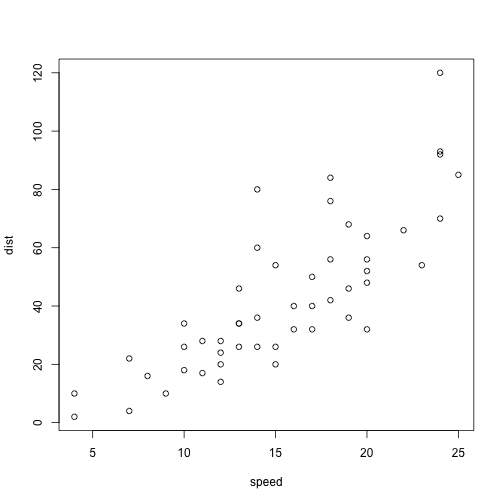
\includegraphics{figure/unnamed-chunk-1.png}
\caption{plot of chunk unnamed-chunk-1}
\end{figure}

\begin{center}\rule{3in}{0.4pt}\end{center}

This report was generated with \href{http://www.r-project.org/}{R}
(2.15.2) and \href{https://github.com/rapporter/pander}{pander} (0.3.1)
on x86\_64-apple-darwin9.8.0 platform.

\end{document}
